% !TeX root = ../../main.tex

\section{Related Work}

Recently, there have been multiple efforts and to scale up deep reinforcement learning, starting with methods that relies on distributed asynchronous SGD~\parencite{dean2012large} with multiple workers. They developed a software framework
called \textbf{DistBelief} that can utilize computing clusters with thousands of machines to train large models. It consists of two main ingredients~\ref{fig:sgd}. First, the parameters of the model can be distributed on multiple servers, depending on the architecture. This set of servers are called the \textit{parameter
servers}. Second, there can be multiple workers processing data in parallel and communicating with the parameter servers. Since each worker communicates with the parameter servers independently of the others, this is
called \textit{Asynchronous Stochastic Gradient Descent} (Async-SGD).

In practice, it means that while a worker computes gradients of the loss with respect to its parameters on a given mini-batch, other workers also interact with the parameter servers and thus potentially update its parameters, hence when a worker sends back its gradients to the parameter server, these gradients are usually computed w.r.t. the parameters of an old version of the model. When a model is trained with N workers, each update will be $N-1$ steps old on average.

\begin{figure}[!htb]
    \centering
    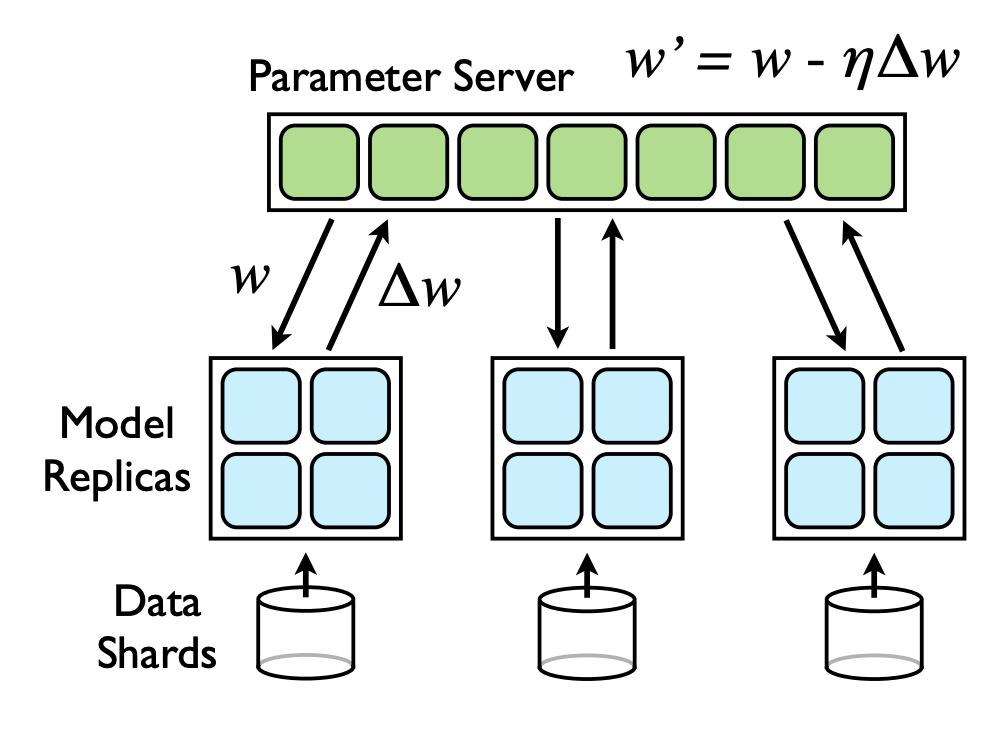
\includegraphics[width=0.5\linewidth]{figures/algos/sgd.png}
    \caption{Async-SGD: Model replicas asynchronously fetch parameters w and push gradients \(\Delta w\) to the parameter server.}
    \label{fig:sgd}
\end{figure}

% \clearpage

Since then a couple of different RL algorithms have proposed including:

$\bullet$ \textit{A distributed version of Deep Q-Networks}~\parencite{ong2015distributed} where they adapt the \textit{DistBelief} software framework to the context of efficiently
training reinforcement learning agents to distribute the deep Q-network training. resulting the method is completely asynchronous and scales well with the number of machines. 

$\bullet$ \textit{Massively parallel methods for DRL}~\ref{fig:gorila} \textbf{(Gorilla)}~\parencite{nair2015massively}, which uses a distributed experience replay buffer (and no prioritization). This architecture~\ref{fig:gorila_arch} uses four main components: \textit{parallel actors} that generate new behaviour, \textit{parallel learners} that are trained from stored experience, \textit{a distributed neural network} to represent the value function or behaviour policy, and \textit{a distributed store of experience} with no prioritization. It was applied to \textbf{49 games} from Atari 2600 games from the Arcade Learning Environment, using identical hyperparameters. The performance~\ref{fig:gorila_results} surpassed \textit{non-distributed DQN} in \textbf{41} of the 49 games and also reduced the wall-time required to achieve these results by an order of magnitude on most games.

\begin{figure}[!htb]
	\centering
	\begin{subfigure}[b]{0.4\textwidth}
		\centering
		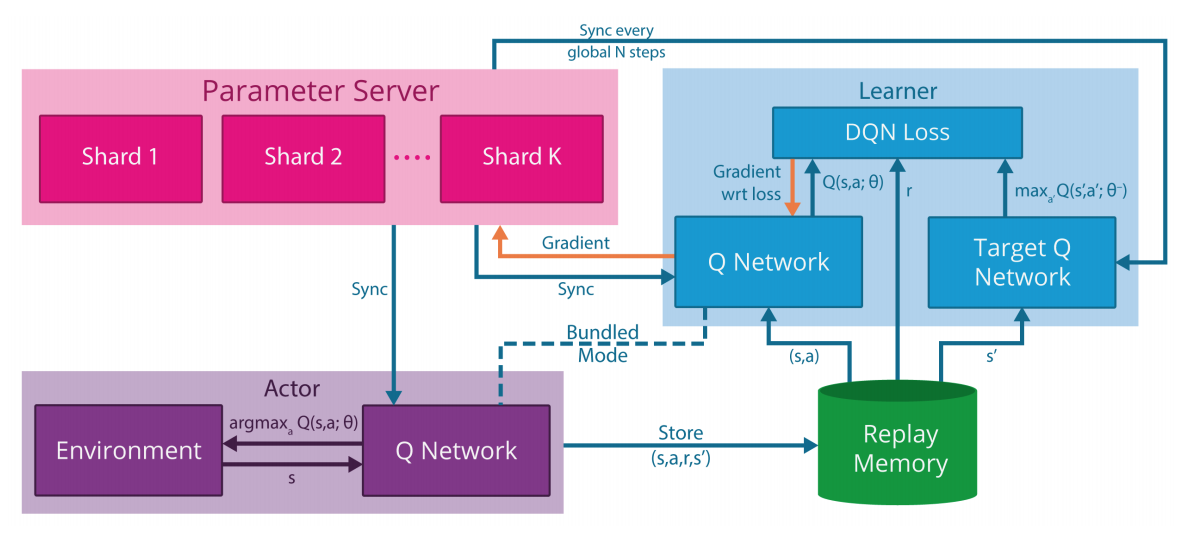
\includegraphics[width=\textwidth]{figures/algos/gorila.png}
		\caption{Agent parallelises the training procedure by separating out learners, actors and parameter server}
		\label{fig:gorila_arch}
    \end{subfigure}
    \hfill
	\begin{subfigure}[b]{0.4\textwidth}
		\centering
		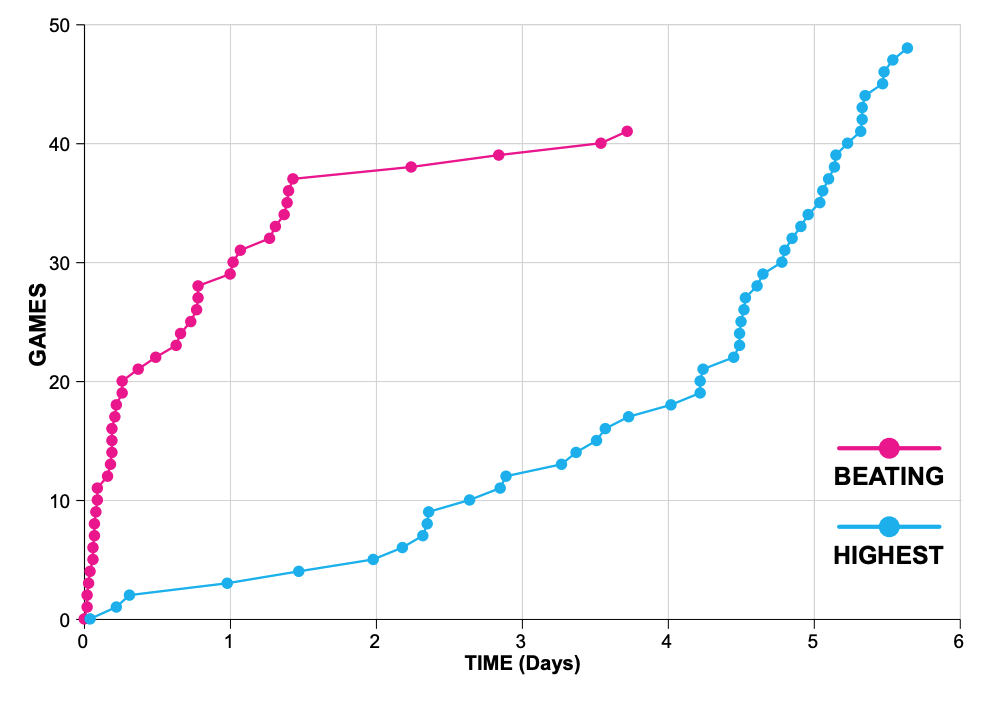
\includegraphics[width=\textwidth]{figures/algos/gorila_results.png}
        \caption{Red curve: time to surpass single DQN\\
                Blue curve: time to reach its peak performance}
		\label{fig:gorila_results}
	\end{subfigure}
	\hfill
	   \caption{The Gorila Architecture \& Results}
	   \label{fig:gorila}
\end{figure}

$\bullet$ \textit{Asynchronous methods for DRL}~\ref{fig:a3c} \textbf{(A3C)}~\parencite{mnih2016asynchronous}, in which they present asynchronous variants of four standard reinforcement learning algorithms and show that parallel actor-learners have a stabilizing effect on training allowing all four methods to successfully train neural network controllers using asynchronous gradient descent for optimization. The algorithms~\ref{fig:a3c_workflow} used multiple threads to run copies of the environment and generate uncorrelated sequences of training samples. Parameters were then sent to a shared parameter server at regular intervals. Because this promotes non-stationarity for the sequences of SARSA tuples, experience replay is not necessarily needed. The implementations of RMSProp and Momentum SGD used by the authors employed a Hogwild-inpsired~\parencite{recht2011hogwild} lock free scheme for maximum efficiency. A3C is the ``best'' agent that was presented in this paper. It is an asynchronous advantage actor-critic algorithm. It maintains an approximation of the policy, an estimate of the value function, and computes an ``advantage'' function and a variance-reducing baseline~\parencite{degris2012off}. An entropy regularization term was also used to discourage premature convergence. The A3C performance overpassed gorila and add some enhancement including faster updates, removing  the replay buffer, and moving to Actor-Critic (from Q learning).

The State-of-the-art results~\ref{fig:a3c_results} were obtained on some of the Atari games (ALE). An LSTM-based A3C agent was tested with Deepmind’s Labyrinth environment. They also tested on the TORCS car racing environment and MuJoCo, the continuous-space physics simulation engine.

\begin{figure}[!htb]
	\centering
	\begin{subfigure}[b]{0.3\textwidth}
		\centering
		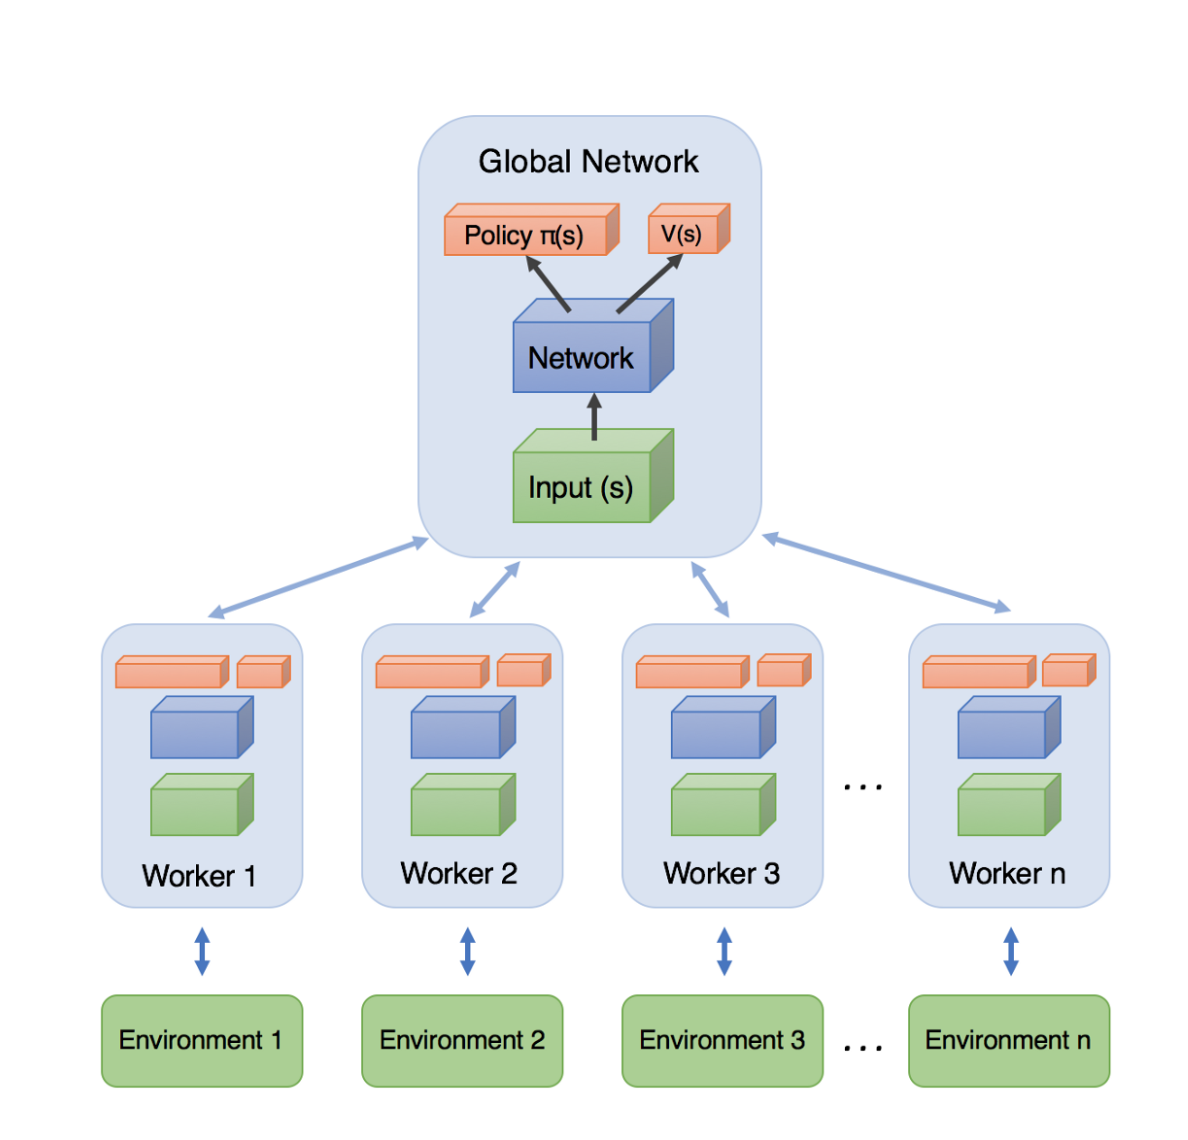
\includegraphics[width=\textwidth]{figures/algos/a3c.png}
		\caption{A3C high-level architecture.}
		\label{fig:a3c_arch}
    \end{subfigure}
    \hfill
    \begin{subfigure}[b]{0.3\textwidth}
		\centering
		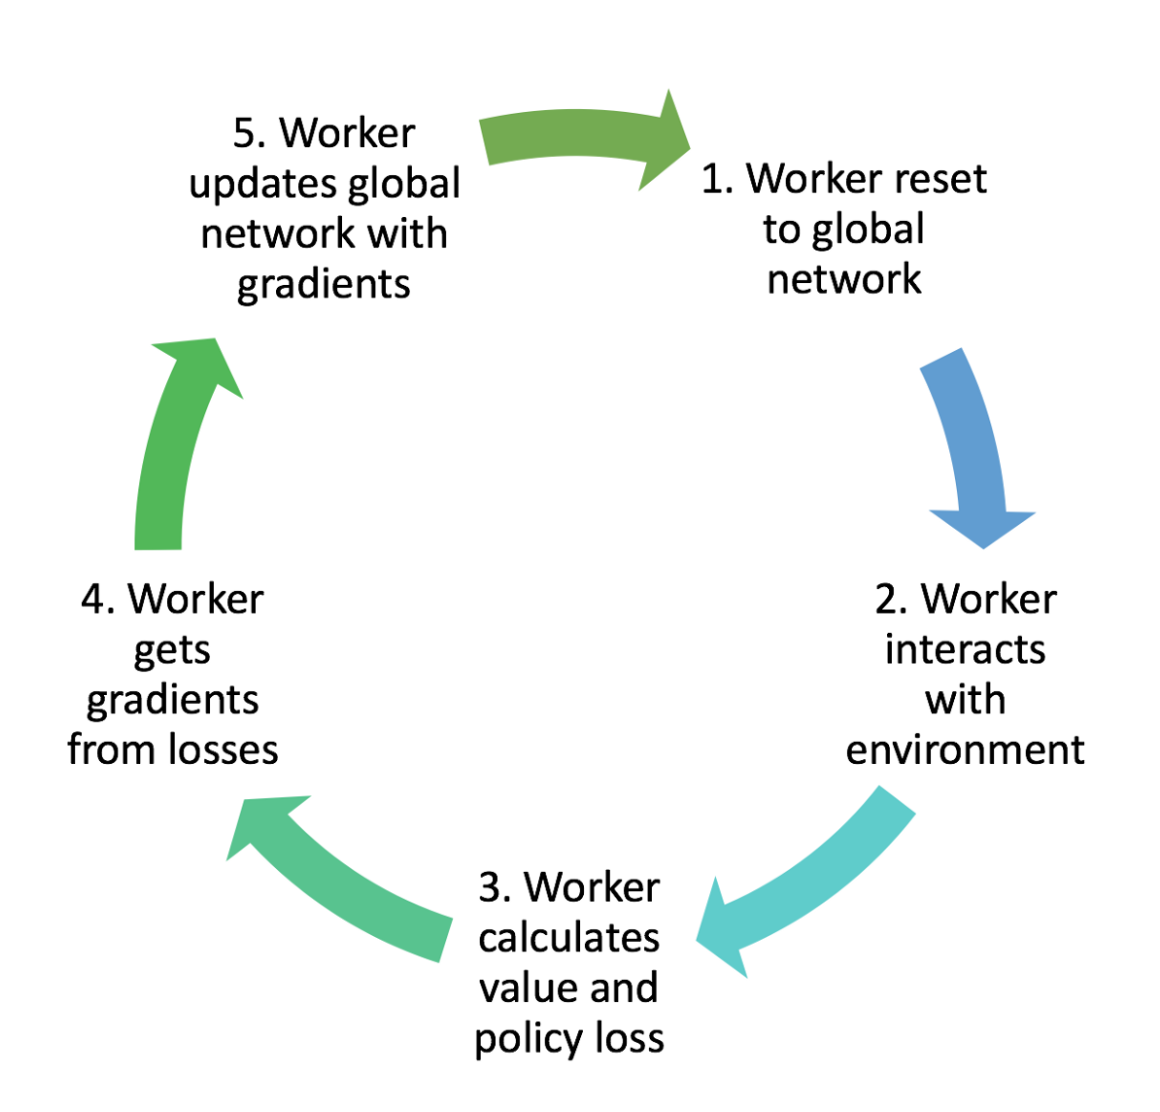
\includegraphics[width=\textwidth]{figures/algos/a3c_workflow.png}
		\caption{Training workflow of each worker agent in A3C.}
		\label{fig:a3c_workflow}
    \end{subfigure}
    \hfill
	\begin{subfigure}[b]{0.3\textwidth}
		\centering
		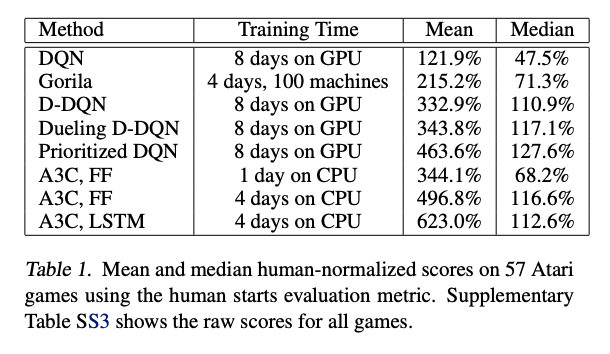
\includegraphics[width=\textwidth]{figures/algos/a3c_results.png}
        \caption{A3C Results}
		\label{fig:a3c_results}
	\end{subfigure}
	\hfill
	   \caption{The A3C Architecture, workflow \& Results}
	   \label{fig:a3c}
\end{figure}

Another direction with some alternatives to \textit{asynchronous SGD} methods which includes distributed BA3C~\parencite{adamski2018distributed}, Evolution strategies~\parencite{salimans2017evolution} using evolutionary processes and 

$\bullet$ \textit{Distributed Prioritized Experience Replay}~\ref{fig:apex} \textbf{(Ape-X)}~\parencite{horgan2018distributed} which use a distributed replay with a synchronous learner. They focused on on applying the Ape-X framework to DQN and DPG, also it could  be combined with any other off-policy reinforcement learning update. 

The main idea of this paper is to scale up the experience replay data by having many actors running in parallel  collect samples of experience. The actors periodically pool their samples into a centralized data repository, which is used for experience replay for a centralized learner to select from it in a prioritized fashion~\parencite{schaul2015prioritized} and update neural network parameters. Those parameters then get copied back to the actors. Hence, they step over and complement standard distributed training approaches~\parencite{dean2012large} of neural networks which focus on parallelizing the computation of gradients to \textit{distribute the generation and selection of experience data}, which suffices to improve results.

This architecture achieved state of the art results~\ref{fig:apex_results} in a wide range of discrete and continuous tasks, both in terms of wall-clock learning speed and final performance

\begin{figure}[!htb]
	\centering
	\begin{subfigure}[b]{0.4\textwidth}
		\centering
		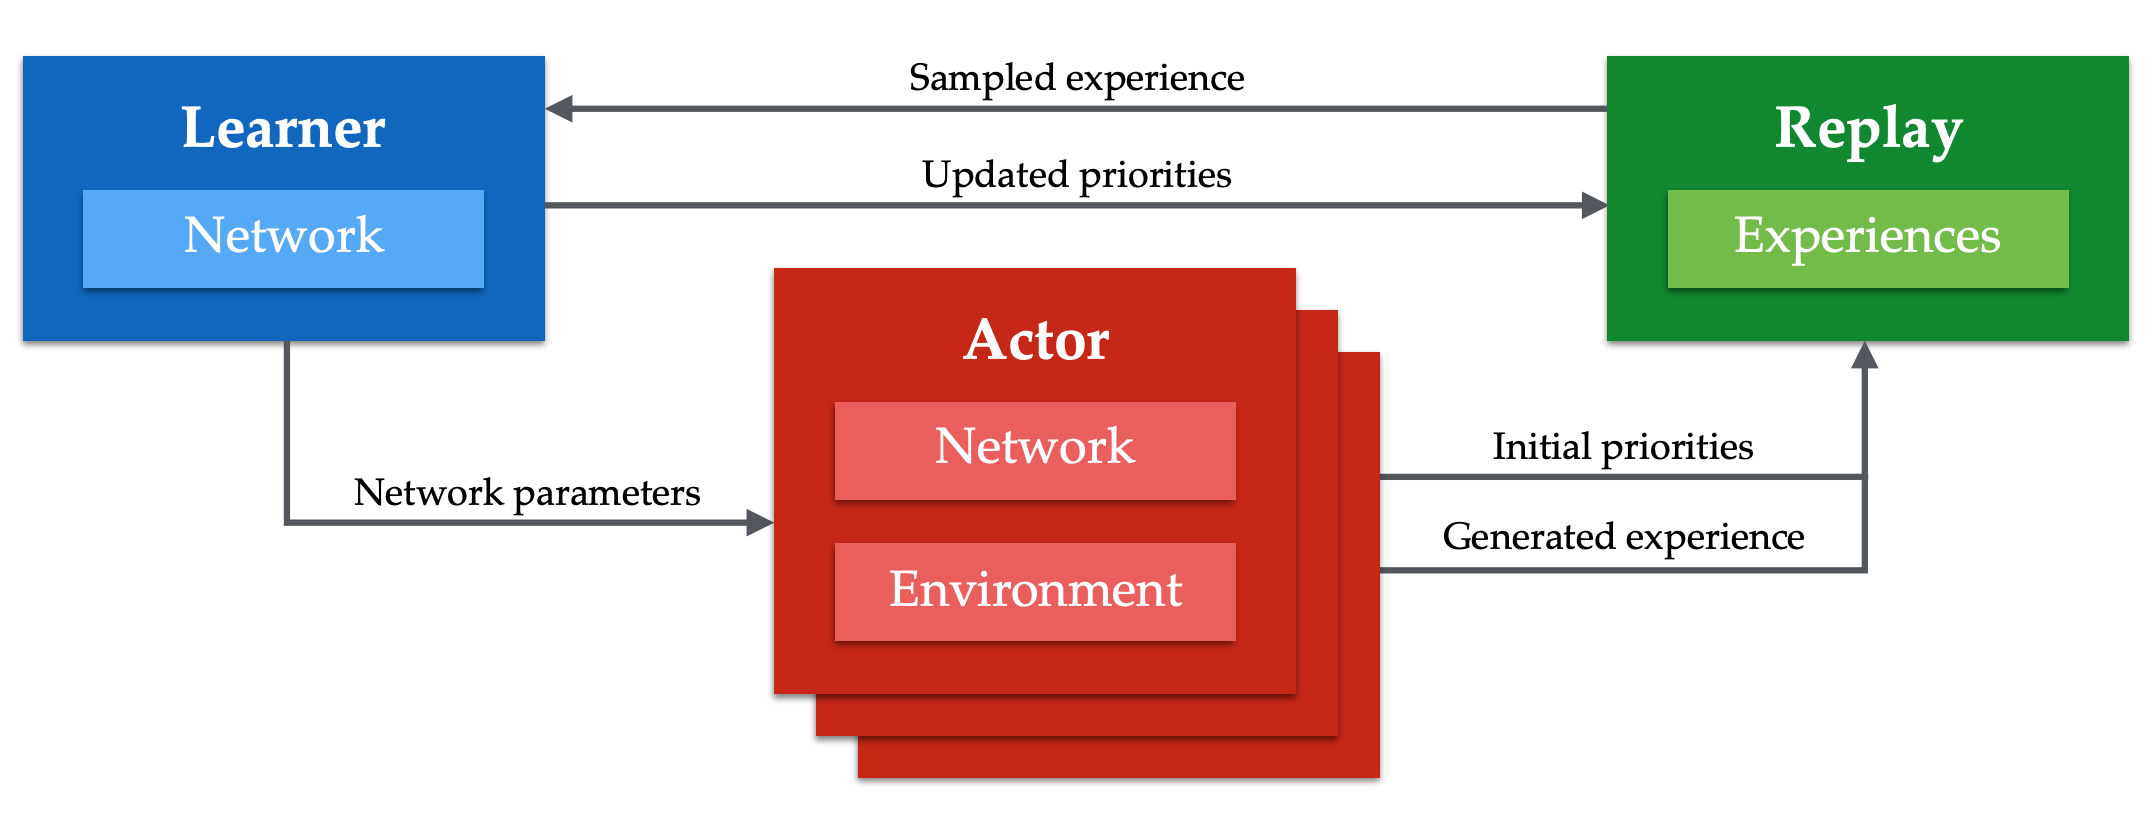
\includegraphics[width=\textwidth]{figures/algos/apex.png}
		\caption{The Ape-X architecture}
		\label{fig:apex_arch}
    \end{subfigure}
    \hfill
	\begin{subfigure}[b]{0.4\textwidth}
		\centering
		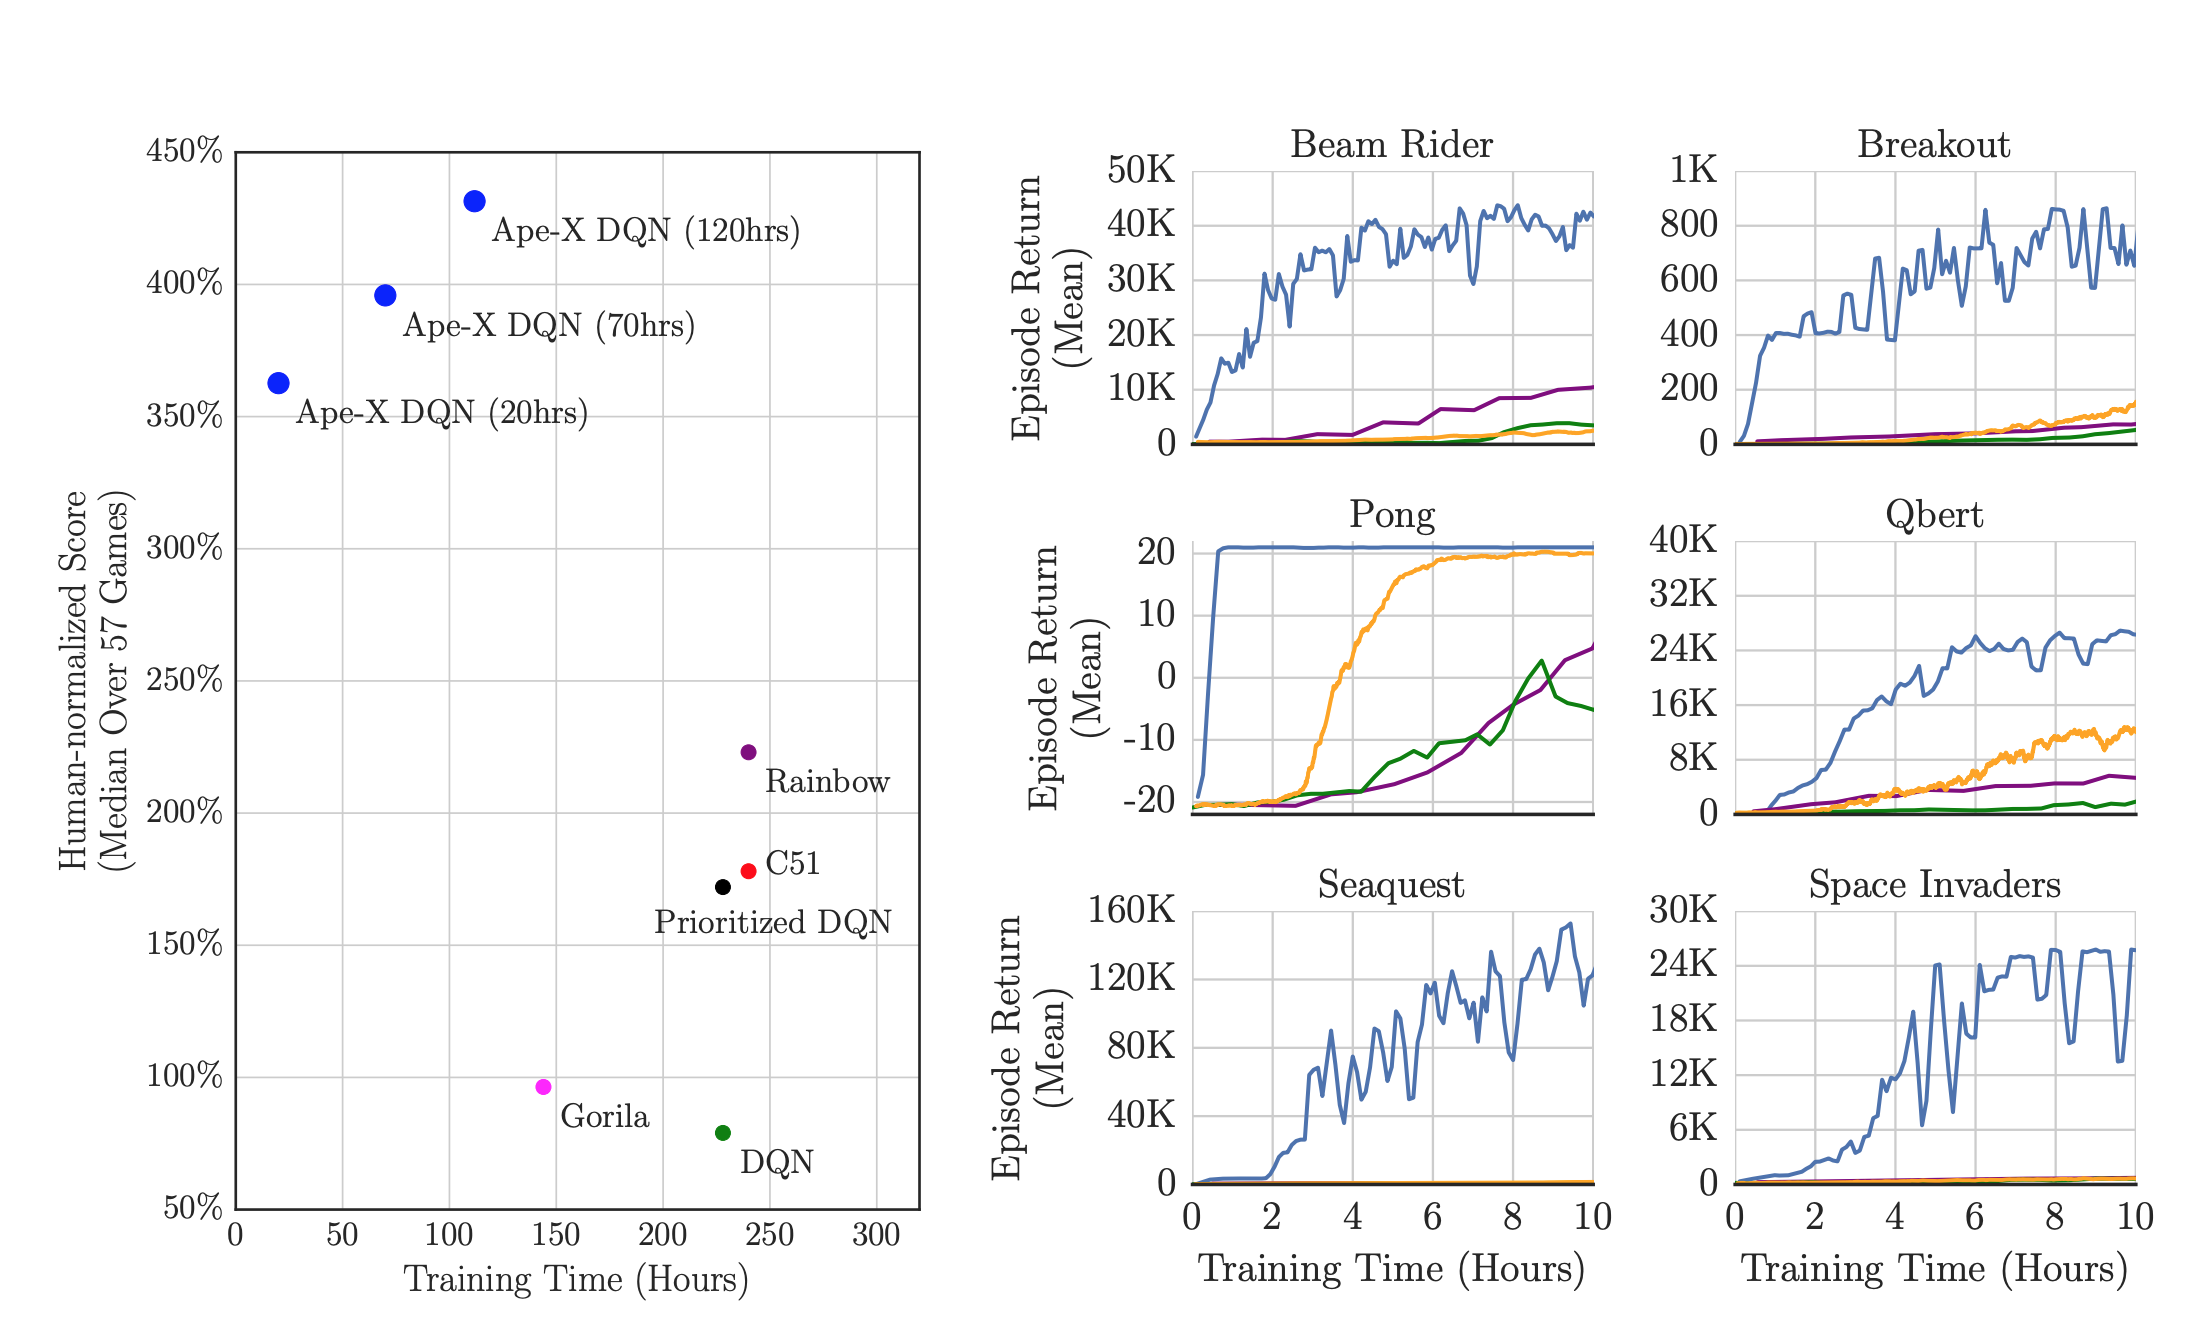
\includegraphics[width=\textwidth]{figures/algos/apex_results.png}
        \caption{Ape-X Performance compared with other RL algorithms}
		\label{fig:apex_results}
	\end{subfigure}
	\hfill
	   \caption{The Ape-X Architecture \& Results}
	   \label{fig:apex}
\end{figure}

Other research have attempt to scale up by using multiple GPUs and utilizing them. The simplest method is batched A2C~\parencite{clemente2017efficient} in which with every step produces a batch of actions and applies them to a batch of environments. BA3C~\parencite{babaeizadeh2016ga3c} another method which uses asynchronous data collection to effectively utilize GPUs.

The most recent work done in the are of distributed deep reinforcement learning and multi-tasking learning which achieve the state of the art performance is \textit{Importance Weighted Actor-Learner Architectures}~\ref{fig:impala} \textbf{(IMPALA)}~\parencite{espeholt2018impala} by DeepMind. It is a scalable distributed DeepRL for their newly designed DMLab-30 environment (which is a collection of new levels designed using our open source RL environment \textit{DeepMind Lab}, These environments are provides to test systems on a large spectrum of interesting tasks either individually or in a multi-task setting).

Importance Weighted Actor-Learner Architecture~\ref{fig:impala_arch} is inspired by the popular \textbf{A3C} architecture which uses multiple distributed actors to learn the agent’s parameters. The developed new distributed agent impala maximizes data throughput using an efficient distributed architecture with TensorFlow. 
In training process for actor-critic methods, each of the actors uses a clone of the policy parameters to act in the environment. Periodically, actors pause their exploration to share the gradients they have computed with a central parameter server that applies updates. 

On the other hand, impala's actors are not used to calculate gradients. Instead, they are just used to \textit{collect experience} which is passed to a \textit{\textbf{central learner}} that computes gradients, resulting in a model that has completely independent actors and learners. 
Separating the learning and acting in this way also has the advantage of increasing the throughput of the whole system since the actors no longer need to wait for the learning step like in architectures such as batched A2C~\ref{fig:impala_vs_a2c}. This allows us to train impala architectures on interesting environments without suffering from variance in frame rendering-time or time consuming task restarts.

However, decoupling the acting and learning causes the policy in the actor to lag behind the learner. In order to compensate for this difference we introduce a principled off-policy advantage actor critic formulation called V-trace which compensates for the trajectories obtained by actors being off policy.

Importance Weighted Actor-Learner Architecture was 10 times more data efficient and achieved double the final score compared to distributed A3C~\ref{fig:impala_results}.  Moreover, Importance Weighted Actor-Learner Architectures showed positive transfer from training in multi-task settings compared to training in single-task setting.

\begin{figure}[!htb]
	\centering
	\begin{subfigure}[b]{0.3\textwidth}
		\centering
		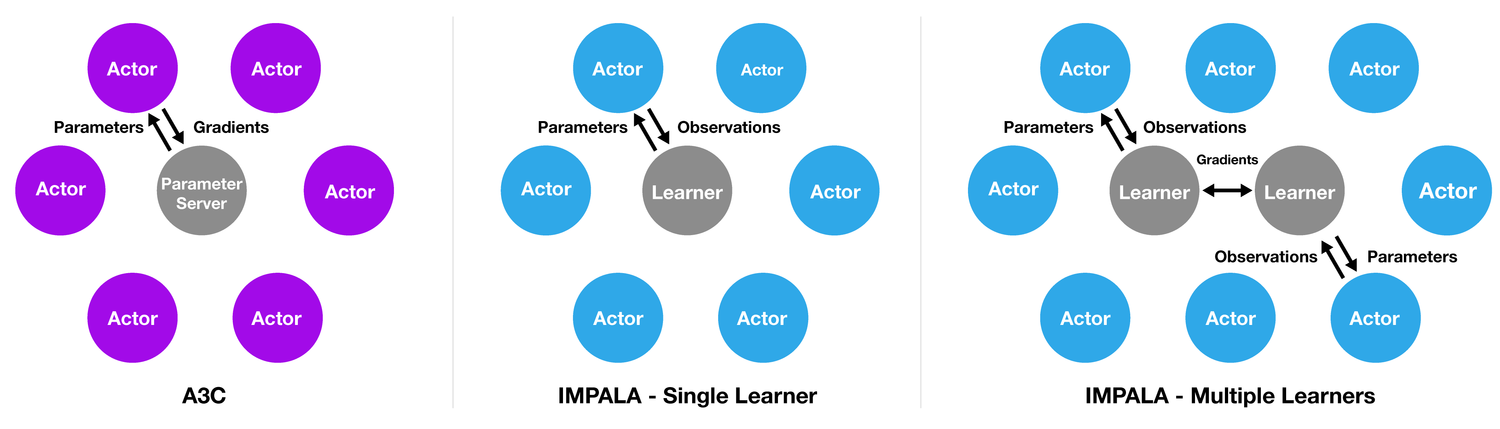
\includegraphics[width=\textwidth]{figures/algos/impala.png}
		\caption{The IMPALA Architecture.}
		\label{fig:impala_arch}
    \end{subfigure}
    \hfill
    \begin{subfigure}[b]{0.3\textwidth}
		\centering
		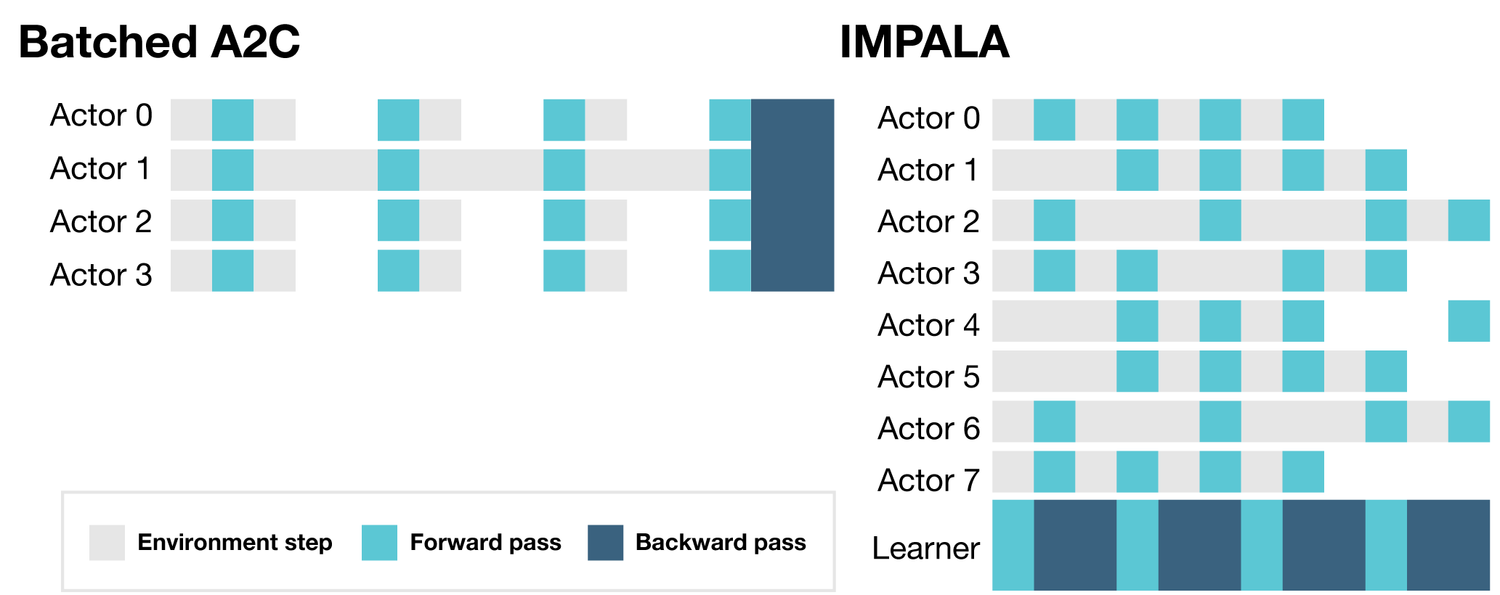
\includegraphics[width=\textwidth]{figures/algos/impala_vs_a2c.png}
		\caption{IMPALA vs Batched A2C Training}
		\label{fig:impala_vs_a2c}
    \end{subfigure}
    \hfill
	\begin{subfigure}[b]{0.3\textwidth}
		\centering
		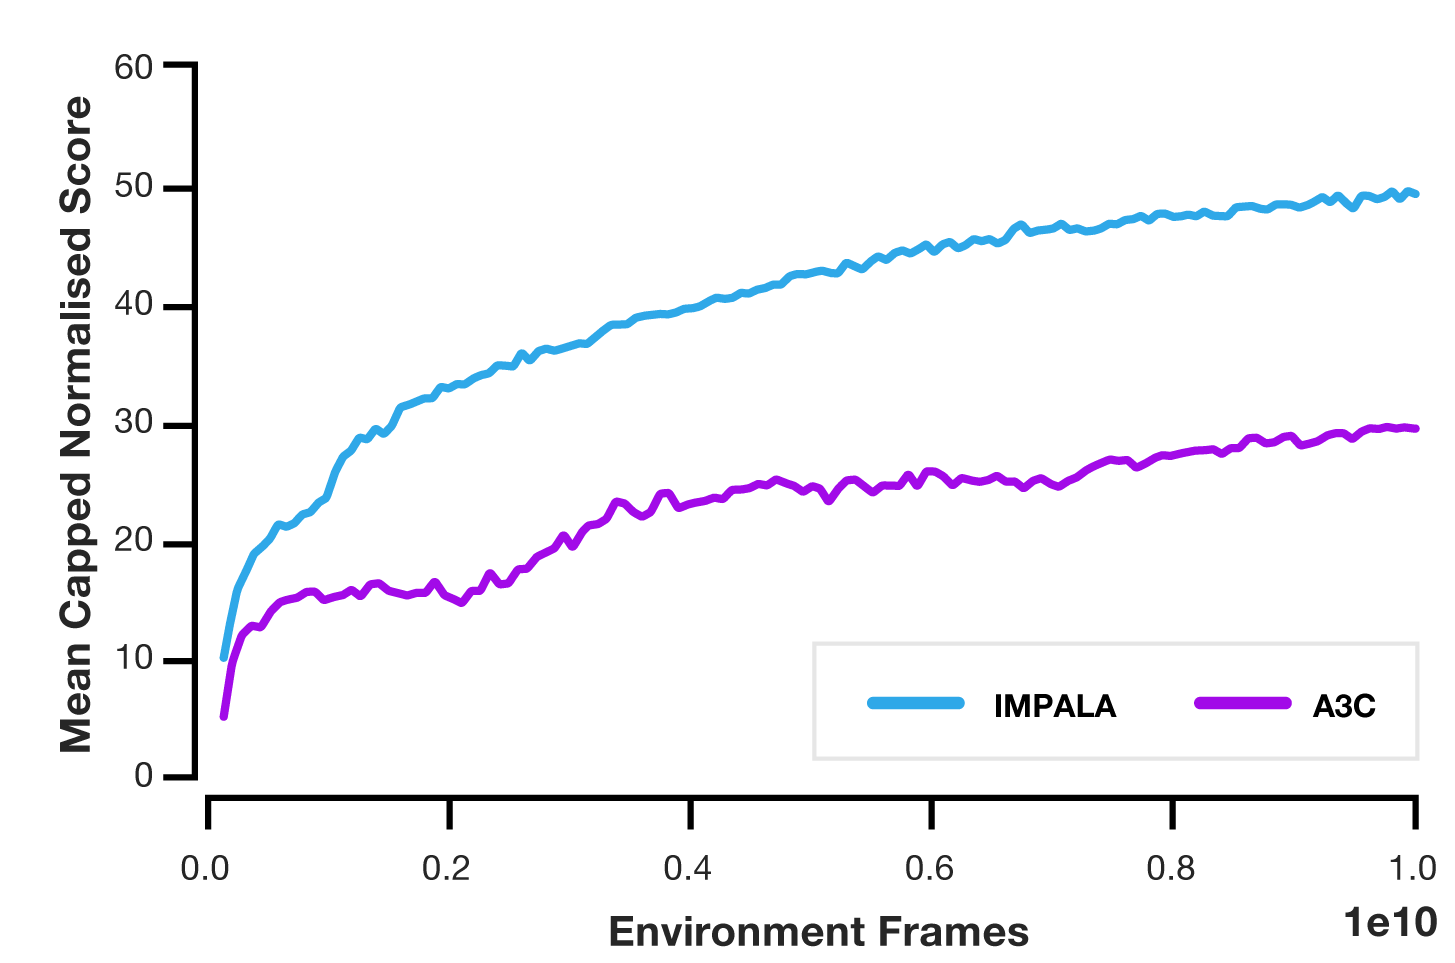
\includegraphics[width=\textwidth]{figures/algos/impala_results.png}
        \caption{IMPALA Results}
		\label{fig:impala_results}
	\end{subfigure}
	\hfill
	   \caption{The IMPALA Architecture, Comparison \& Results}
	   \label{fig:impala}
\end{figure}

On the practical side, there have been some frameworks developments that focuses on distributed deep reinforcement learning and applying all the techniques and algorithms to multiple environments for the sake of advancing DRL research. Dopamine~\parencite{castro2018dopamine} is a new framework for flexible and reproducible Reinforcement Learning Research by google in which they provide large-scale distributed training and enabling distributing the learning process across multiple workers, with distributional methods that allow agents to model full distributions, rather than simply their expected values, to learn a more complete picture of their world. This framework aims to provide flexibility, stability, and reproducibility for new and experienced RL researchers alike. Inspired by one of the main components in \textit{reward-motivated behaviour (dopamine)} in the brain and reflecting the strong historical connection between neuroscience and reinforcement learning research.

Ray~\parencite{moritz2018ray} is another more general framework with Distributed Execution for AI Applications. Ray is a high-performance distributed execution framework targeted at large-scale machine learning and reinforcement learning applications. It achieves scalability and fault tolerance by abstracting the control state of the system in a global control store and keeping all other components stateless. It uses a shared-memory distributed object store to efficiently handle large data through shared memory, and it uses a bottom-up hierarchical scheduling architecture to achieve low-latency and high-throughput scheduling. It uses a lightweight API based on dynamic task graphs and actors to express a wide range of applications in a flexible manner.
